Baking refers to the part of the process where you are loading
your dough into the oven. This is typically done after your
dough has gone through the bulk fermentation and proofing stage.

\begin{figure}[!htb]
  \begin{tikzpicture}[node distance = 3cm, auto]
    \node [block] (heat_oven) {\footnotesize Heat oven to 230°C (446°F) for 30 minutes};
    \node [block, right of=heat_oven, node distance=3cm] (score_dough) {\footnotesize Score your dough};
    \node [decision, right of=score_dough, node distance=4cm] (decide_steam) {\footnotesize Choose your steaming method};
    \node [block, below of=heat_oven, node distance=4cm] (inverted_tray_method) {\footnotesize Inverted tray method};
    \node [block, right of=inverted_tray_method, node distance=3cm] (dutch_oven) {\footnotesize Dutch oven};
    \node [block, right of=dutch_oven, node distance=3cm] (steam_injection) {\footnotesize Steam injection oven};
    \node [block, below of=inverted_tray_method, node distance=3cm] (bake_30) {\footnotesize Bake dough for 30 minutes with steam};
    \node [block, right of=bake_30, node distance=3cm] (remove_steam) {\footnotesize Remove source of steam};
    \node [block, right of=remove_steam, node distance=3cm] (build_crust) {\footnotesize Build the crust};
    \node [block, right of=build_crust, node distance=3cm] (finish_baking) {\footnotesize Stop baking 10-30 minutes later depending on crust preference};
    \path [line] (heat_oven) -- (score_dough);
    \path [line] (score_dough) -- (decide_steam);
    \path [line] (decide_steam) -- (inverted_tray_method);
    \path [line] (decide_steam) -- (dutch_oven);
    \path [line] (decide_steam) -- (steam_injection);
    \path [line] (steam_injection) -- (bake_30);
    \path [line] (inverted_tray_method) -- (bake_30);
    \path [line] (dutch_oven) -- (bake_30);
    \path [line] (bake_30) -- (remove_steam);
    \path [line] (remove_steam) -- (build_crust);
    \path [line] (build_crust) -- (finish_baking);
  \end{tikzpicture}
  \caption{A schematic visualization of the baking process using different sources of steam in a home oven.}
  \label{fig:baking-process}
\end{figure}

Some other breads like flat breads
could also be baked on the stove. This chapter is focusing on the
home oven though.

As the dough heats up the the water and acids
in your dough start to evaporate. When baking
a gluten based dough the bubbles in your dough start to expand.
Your dough starts to vertically rise. This is called oven spring.
Your bread starts to build a crust of gel like consistency. The crust is still
extensible and can be stretched.

\begin{table}[!htb]
  \centering
  \resizebox{\textwidth}{!}{%
  \begin{tabular}{|l|l|l|}
  \hline
  \textbf{°C  °F} & \textbf{Stage}         & \textbf{Description}                                                                                                                                           \\ \hline
  60 - 140        & Sterilisation          & \begin{tabular}[c]{@{}l@{}}The temperature is too hot for your\\ microorganisms and they die\end{tabular}                                                      \\ \hline
  75 - 167        & Gel building           & \begin{tabular}[c]{@{}l@{}}A gel builds on the surface persisting\\ your dough's structure. It is still\\ extensible and can spring in the\\ oven\end{tabular} \\ \hline
  100 - 212       & Water evaporates       & \begin{tabular}[c]{@{}l@{}}Water begins to evaporate and\\ inflates your dough's alveoli\end{tabular}                                                          \\ \hline
  118 - 244       & Acetic acid evaporates & \begin{tabular}[c]{@{}l@{}}The vinegary tasting acid starts\\ to evaporate. The sourness decreases\end{tabular}                                                \\ \hline
  122 - 252       & Lactic acid evaporates & \begin{tabular}[c]{@{}l@{}}The dairy tasting lactic acid begins\\ to evaporate. Sourness further decreases\end{tabular}                                        \\ \hline
  140 - 284       & Maillard reaction      & \begin{tabular}[c]{@{}l@{}}The maillard reaction starts to deform\\ starches and proteins. The dough starts\\ browning\end{tabular}                            \\ \hline
  170 - 338       & Caramelization         & \begin{tabular}[c]{@{}l@{}}Remaining sugars begin to caramelise\\ giving your bread a distinct flavor\end{tabular}                                             \\ \hline
  \end{tabular}%
  }
  \caption{The different stages of the baking process and their impact on your bread}
\end{table}

At around 60°C (140°F) the microbes in your dough start to die.
There are rumors that until this happens the microbes produce
a lot of CO2, resulting in the dough's expansion. This temperature
is however reached quickly. Furthermore stress makes the microbes
enter sporulation mode in order to focus on spreading genetics.
More research should be done here to validate or invalidate this
claim.

At 75°C (167°F) the surface of your dough turns into a gel. It
holds together nicely and is still extensible. This gel is essential
for oven spring as it retains the gas of your dough very well.

At around 100°C (212°F) the water starts to evaporate out of your
dough. If this wasn't the case your dough would taste soggy and
doughy. The higher hydration your dough has the more water your bread
still contains after the bake. The crumb is going to taste a bit
more moist. The consistency will be different.

Another often undervalued step is the evaporation of acids. At
118°C (244°F) the acetic acid in your dough starters to evaporate.
Shortly after at 122°C (252°F) the lactic acid begins evaporating.
This is crucial to understand and opens a door to many interesting
ways to influence your final bread's taste. As more and more water
begins to evaporate the acids in your dough become more concentrated.
There is less water but in relation you have more acids. So a shorter
bake will lead to a more tangy dough. The longer you bake the bread
the more of the water evaporates, but also ultimately the acids will follow.
They will be more concentrated. In absolute units though they
will become less and less. The longer you bake the less sour
your bread is going to be. So by baking you can
influence which sourness level you would like to achieve.

\begin{figure}[!htb]
  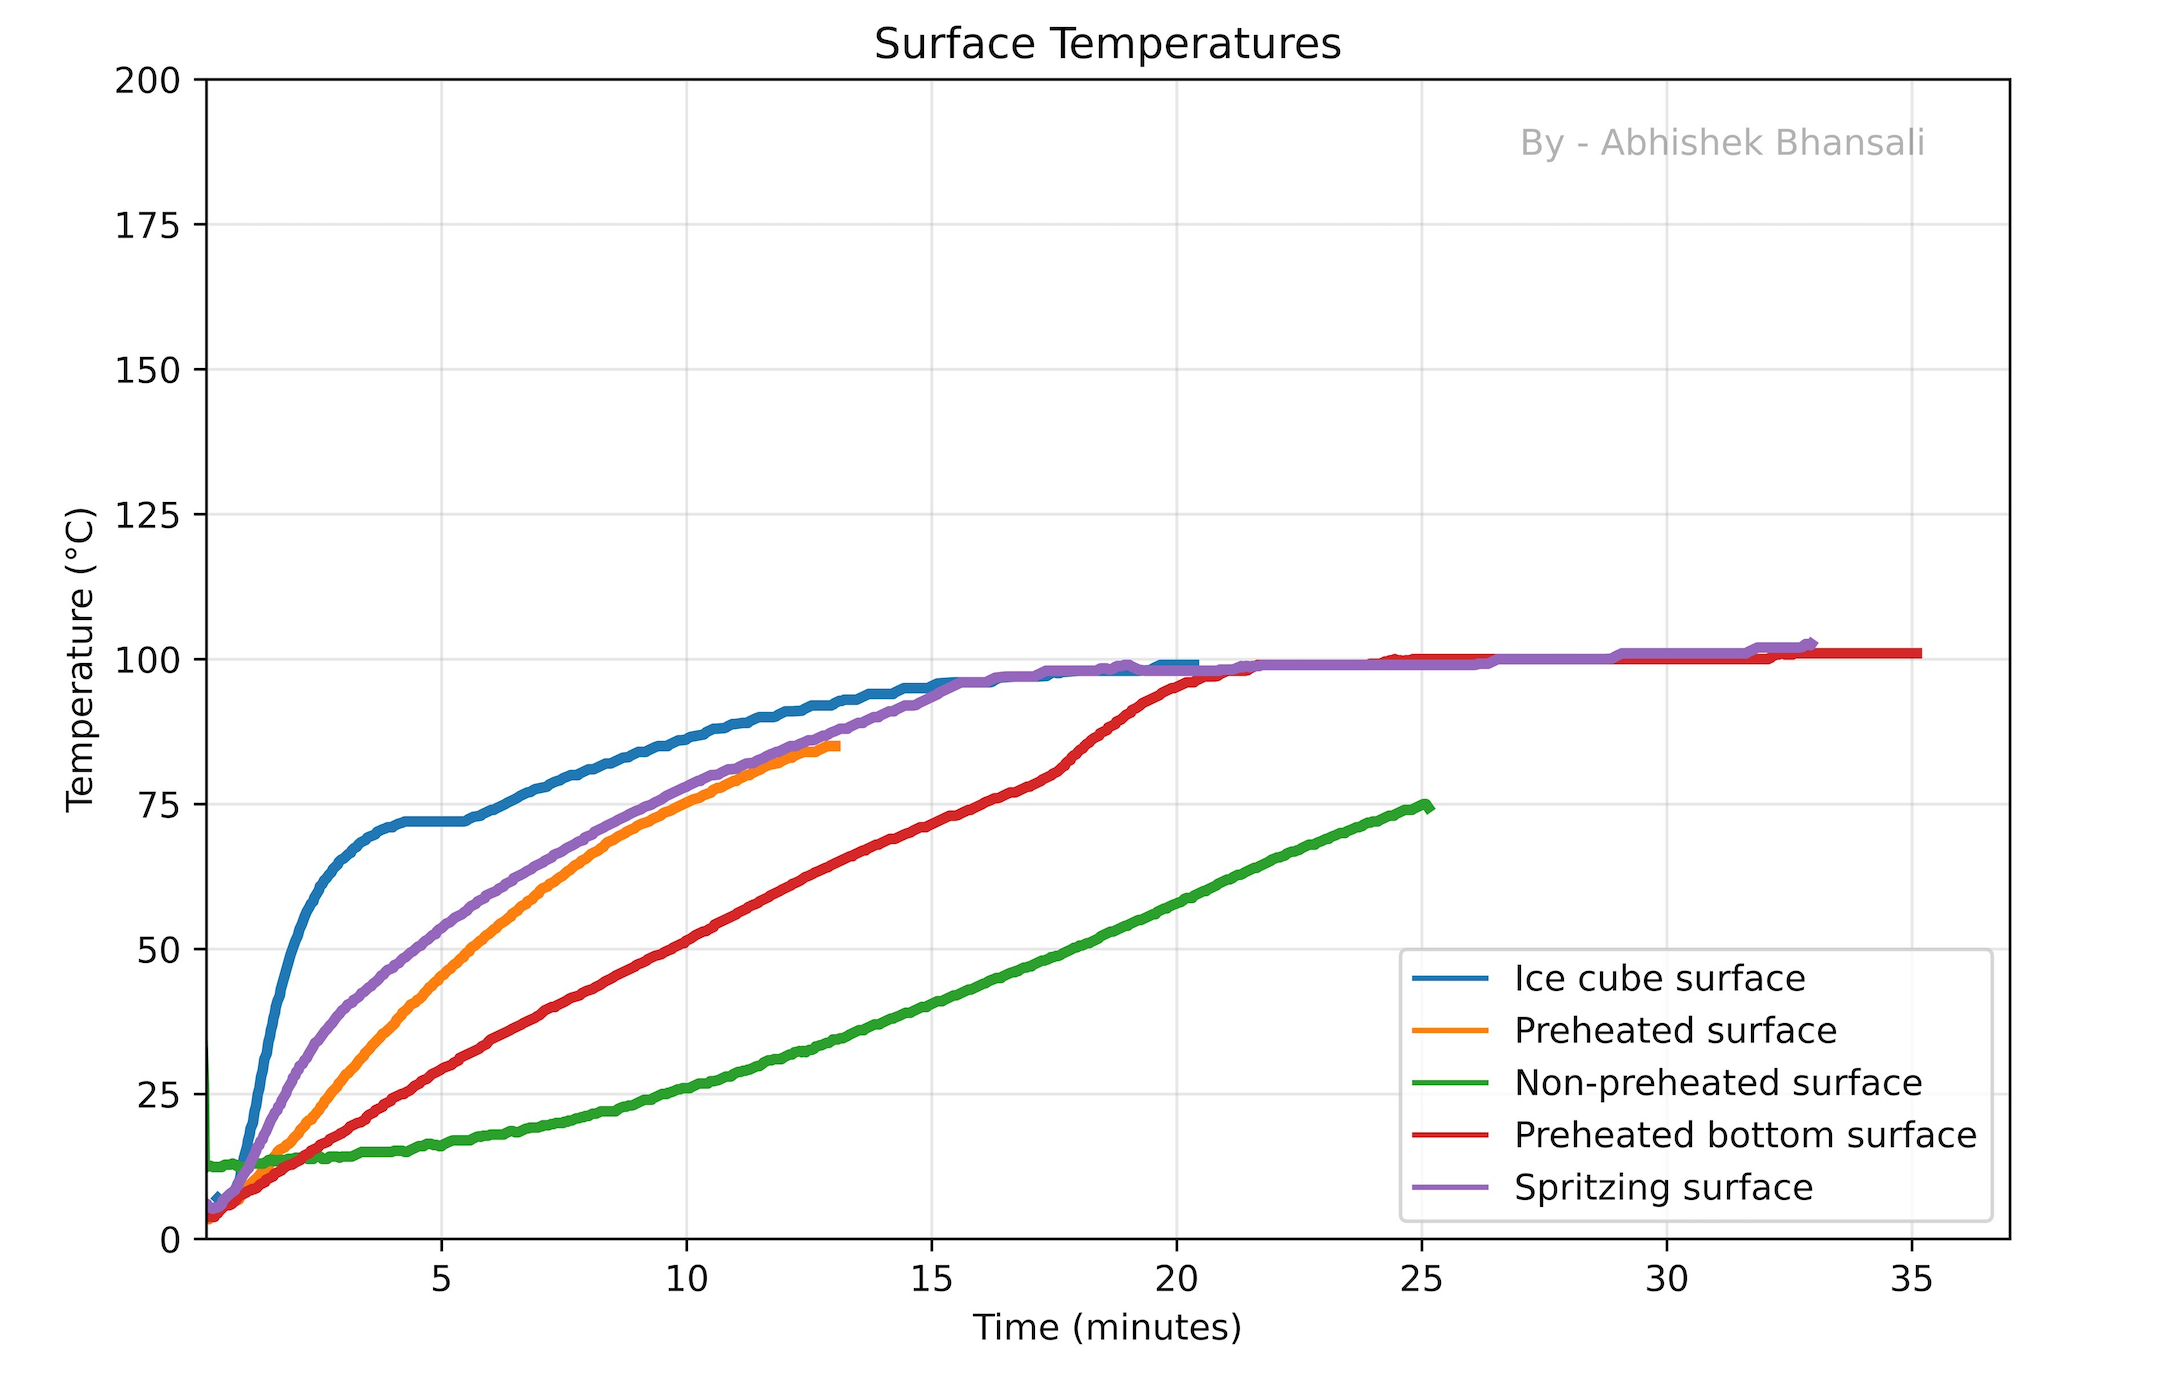
\includegraphics[width=\textwidth]{baking-experiment-temperatures.png}
  \caption{This chart shows how surface temperatures change using
  different steaming methods. In this case I used a dutch oven and an apple as
  dough replacement. All the apples were coming from the fridge. The temperature
  was measured using a barbecue thermometer.
  The more steam the faster the surface temperature increases.}
\end{figure}

It would be a very interesting experiment to bake a bread at different exact
temperatures. How would a bread taste with only evaporated water but
full acidity? What if you were to just completely get rid of the acetic
acid? How would the taste change?

As the temperature increases
the crust thickens. The maillard reaction kicks in further deforming
proteins and starches. The outside of your dough starts to become
browner and crisper. This process begins at around 140°C (284°F)

Once the temperature increases even more to around 170°C (338°F)
the caramelization process begins. The remaining sugars the microbes
did not convert yet start to brown and darken. You can keep baking
for as long as you like to achieve the crust color that you like.
\footnote{This really depends a lot on your personal preference.
Some people prefer a darker crust, others prefer a more pale crust.
It's better to build less crust than too much. You can always just
heat your bread in the oven one more time to continue building a
darker crust.}

The best option to know that your dough is done is to take
the temperature of your dough. You can use a barbecue thermometer
to measure it. Once the core temperature is at around 92°C (197°F)
you can stop the baking process. This is typically not done though
as the crust hasn't been built yet.\footnote{The thermometer is
especially important when using a large loaf pan. It is sometimes
very hard to judge from the outside if the dough is done. I failed
many times and ended up having a semi baked dough.}

Once your dough has finished baking it is ready to eat. Your
dough has turned into a bread. At this
point your bread is sterile as the temperature was too hot for
for the microorganisms to survive.

\section{The role of steam}

Steam is essential when baking as it helps to counter premature
crust building. During the first stage of the bake the dough
increases in size. The water in your dough evaporates and pushes
the whole dough upwards. 

\begin{figure}[!htb]
  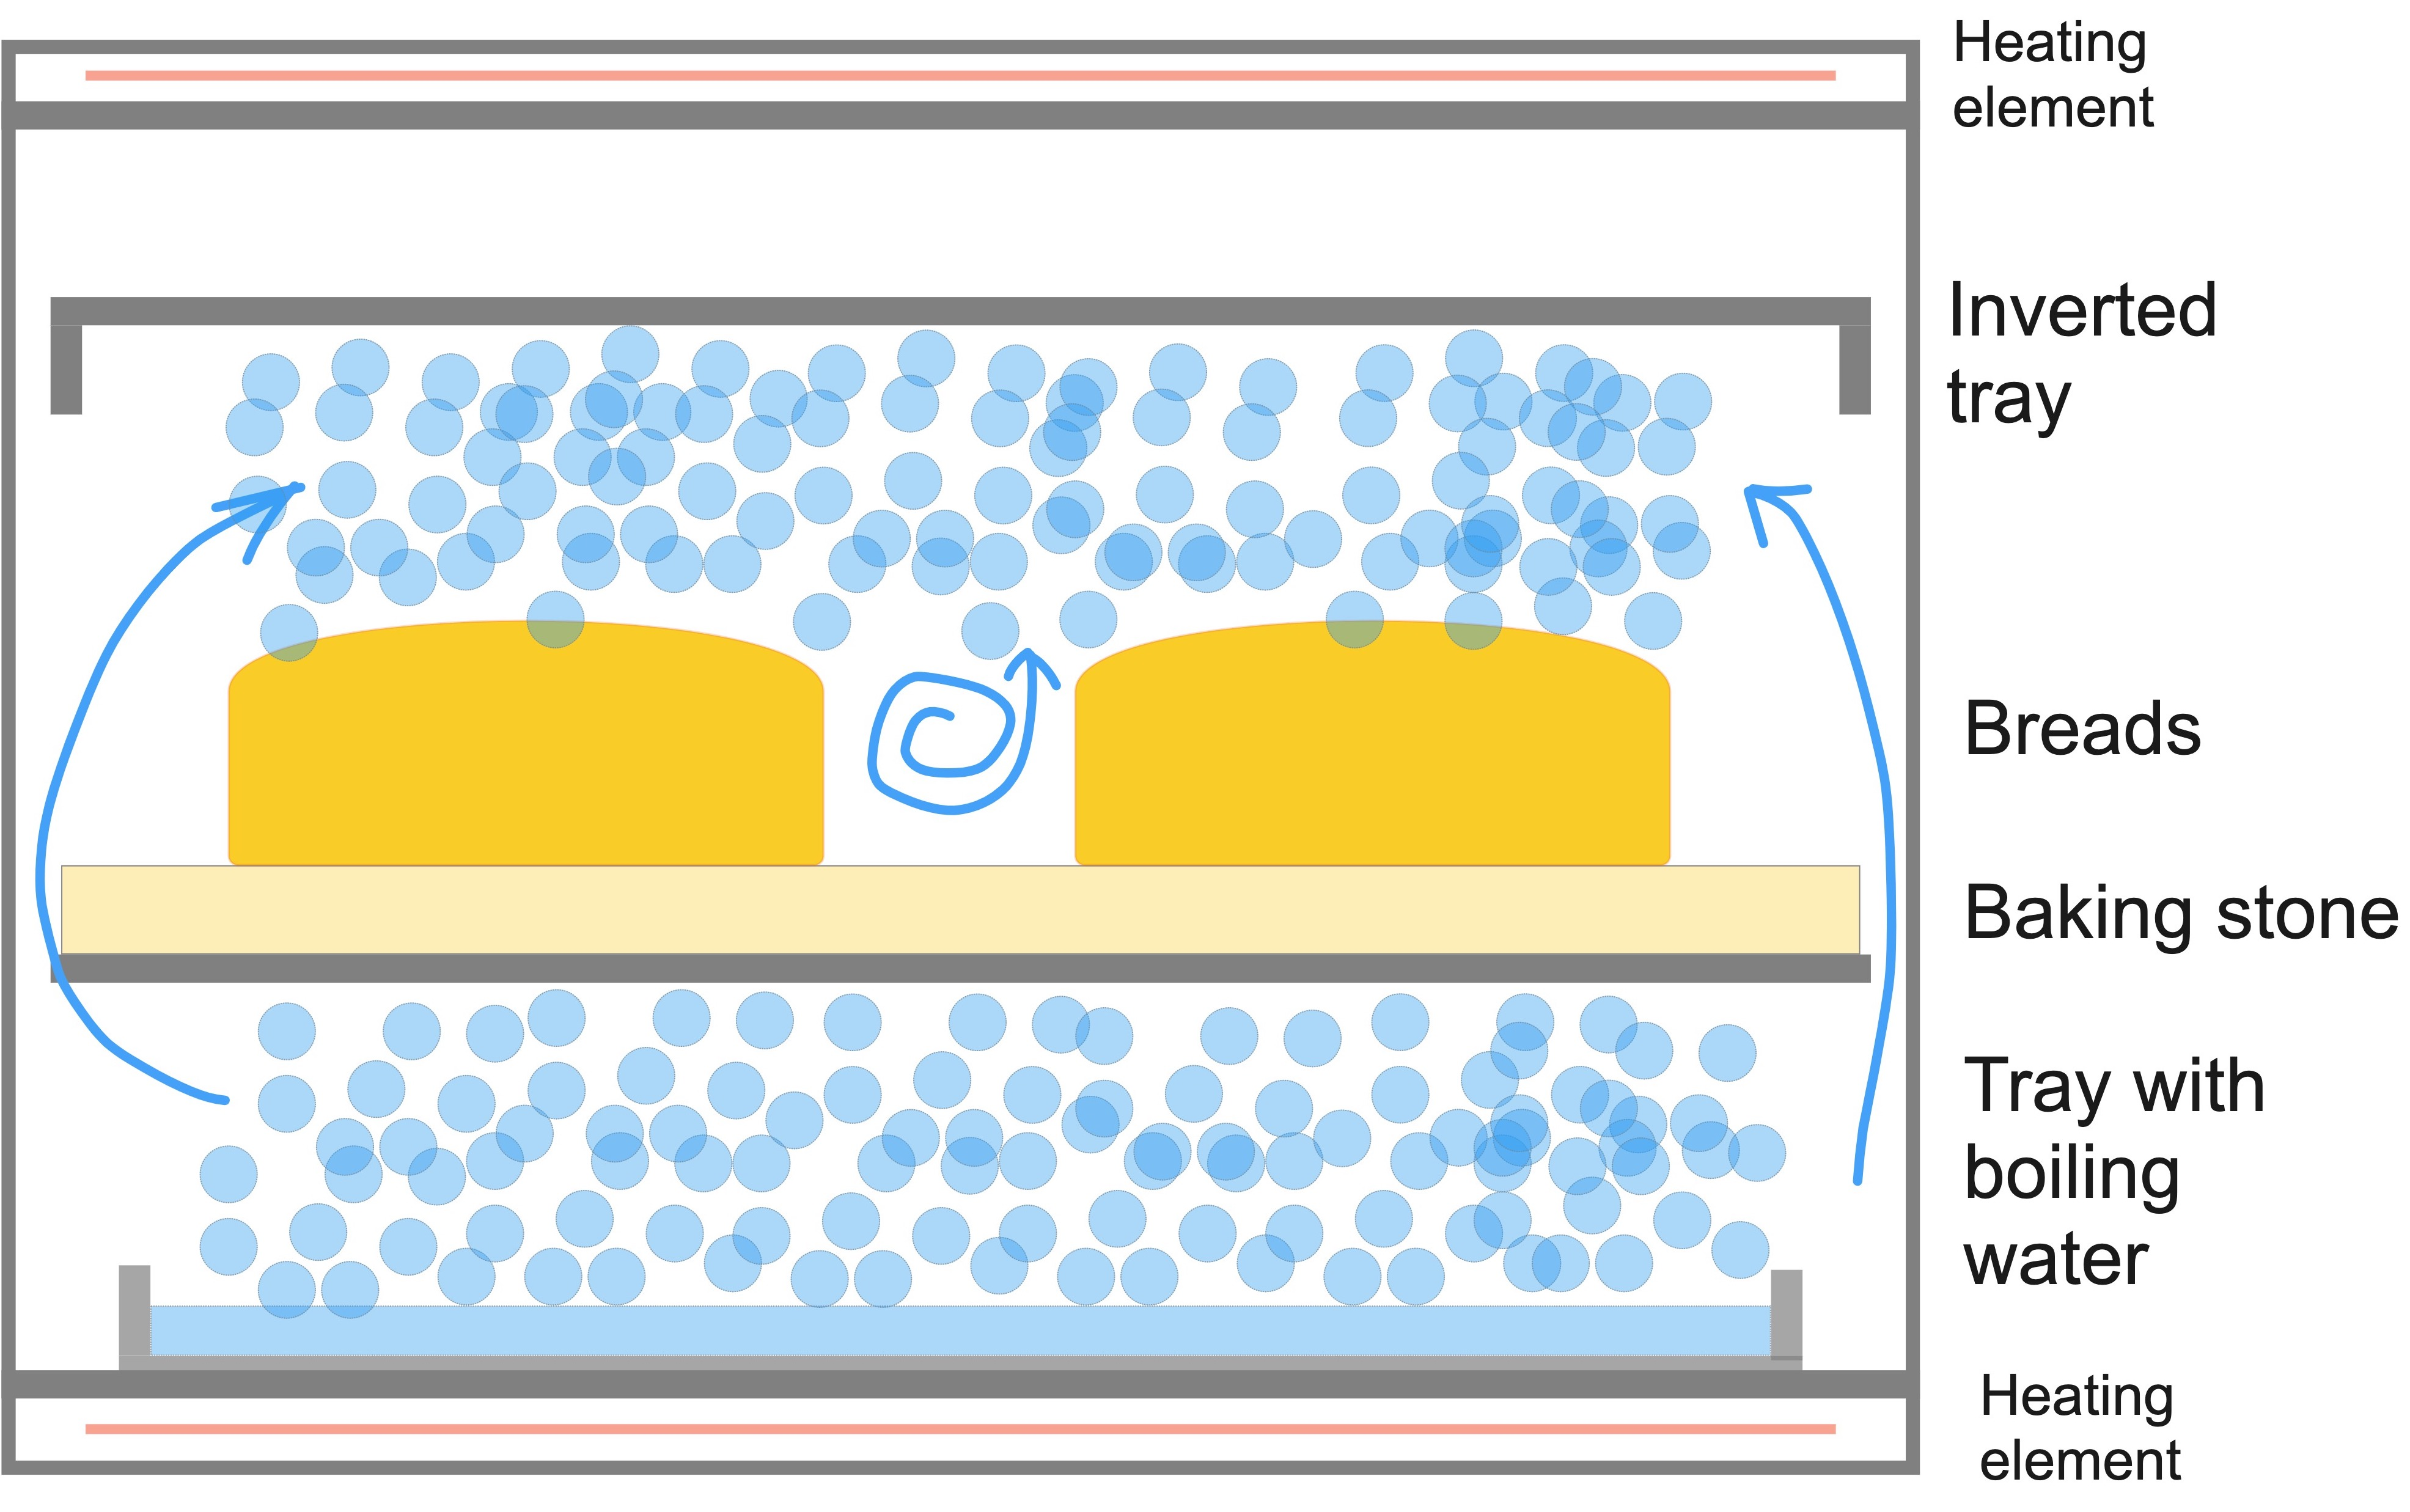
\includegraphics[width=\textwidth]{baking-process-steam.jpg}
  \caption{How steam builds in your oven using the later described
  inverted tray method}
\end{figure}

Normally under high heat a crust would form. Just like
if you were to bake vegetables in your home oven. At some point
they become darker and crisper. This is the same thing that
happens with your dough. You want to delay this process
as long as possible until your dough no longer expands.
Expansion stops when most of the microbes have died and
the evaporating water no longer stays inside the alveoli.
The stronger the gluten network the more gas can be retained
during the baking process. This gluten network at some point
loses its ability to contain gas as the temperature heats
up. The dough stops to increase in size. The steam plays
an important role as it condenses and evaporates on top
of your dough. The surface temperature is rapidly increasing
to around 75°C (160°F). At this temperature the gel starts
to build. This gel is still extensible and allows expansion.
Without the steam the dough would never enter the gel stage,
but instead directly go to the maillard reaction zone. You
want your dough to stay in this gel stage as long as possible
to achieve maximum expansion.\footnote{You can remove your
dough from the oven after 5 minutes to see the gel. You will notice
that it holds the doughs structure. It has a very interesting consistency.}

\begin{figure}[!htb]
  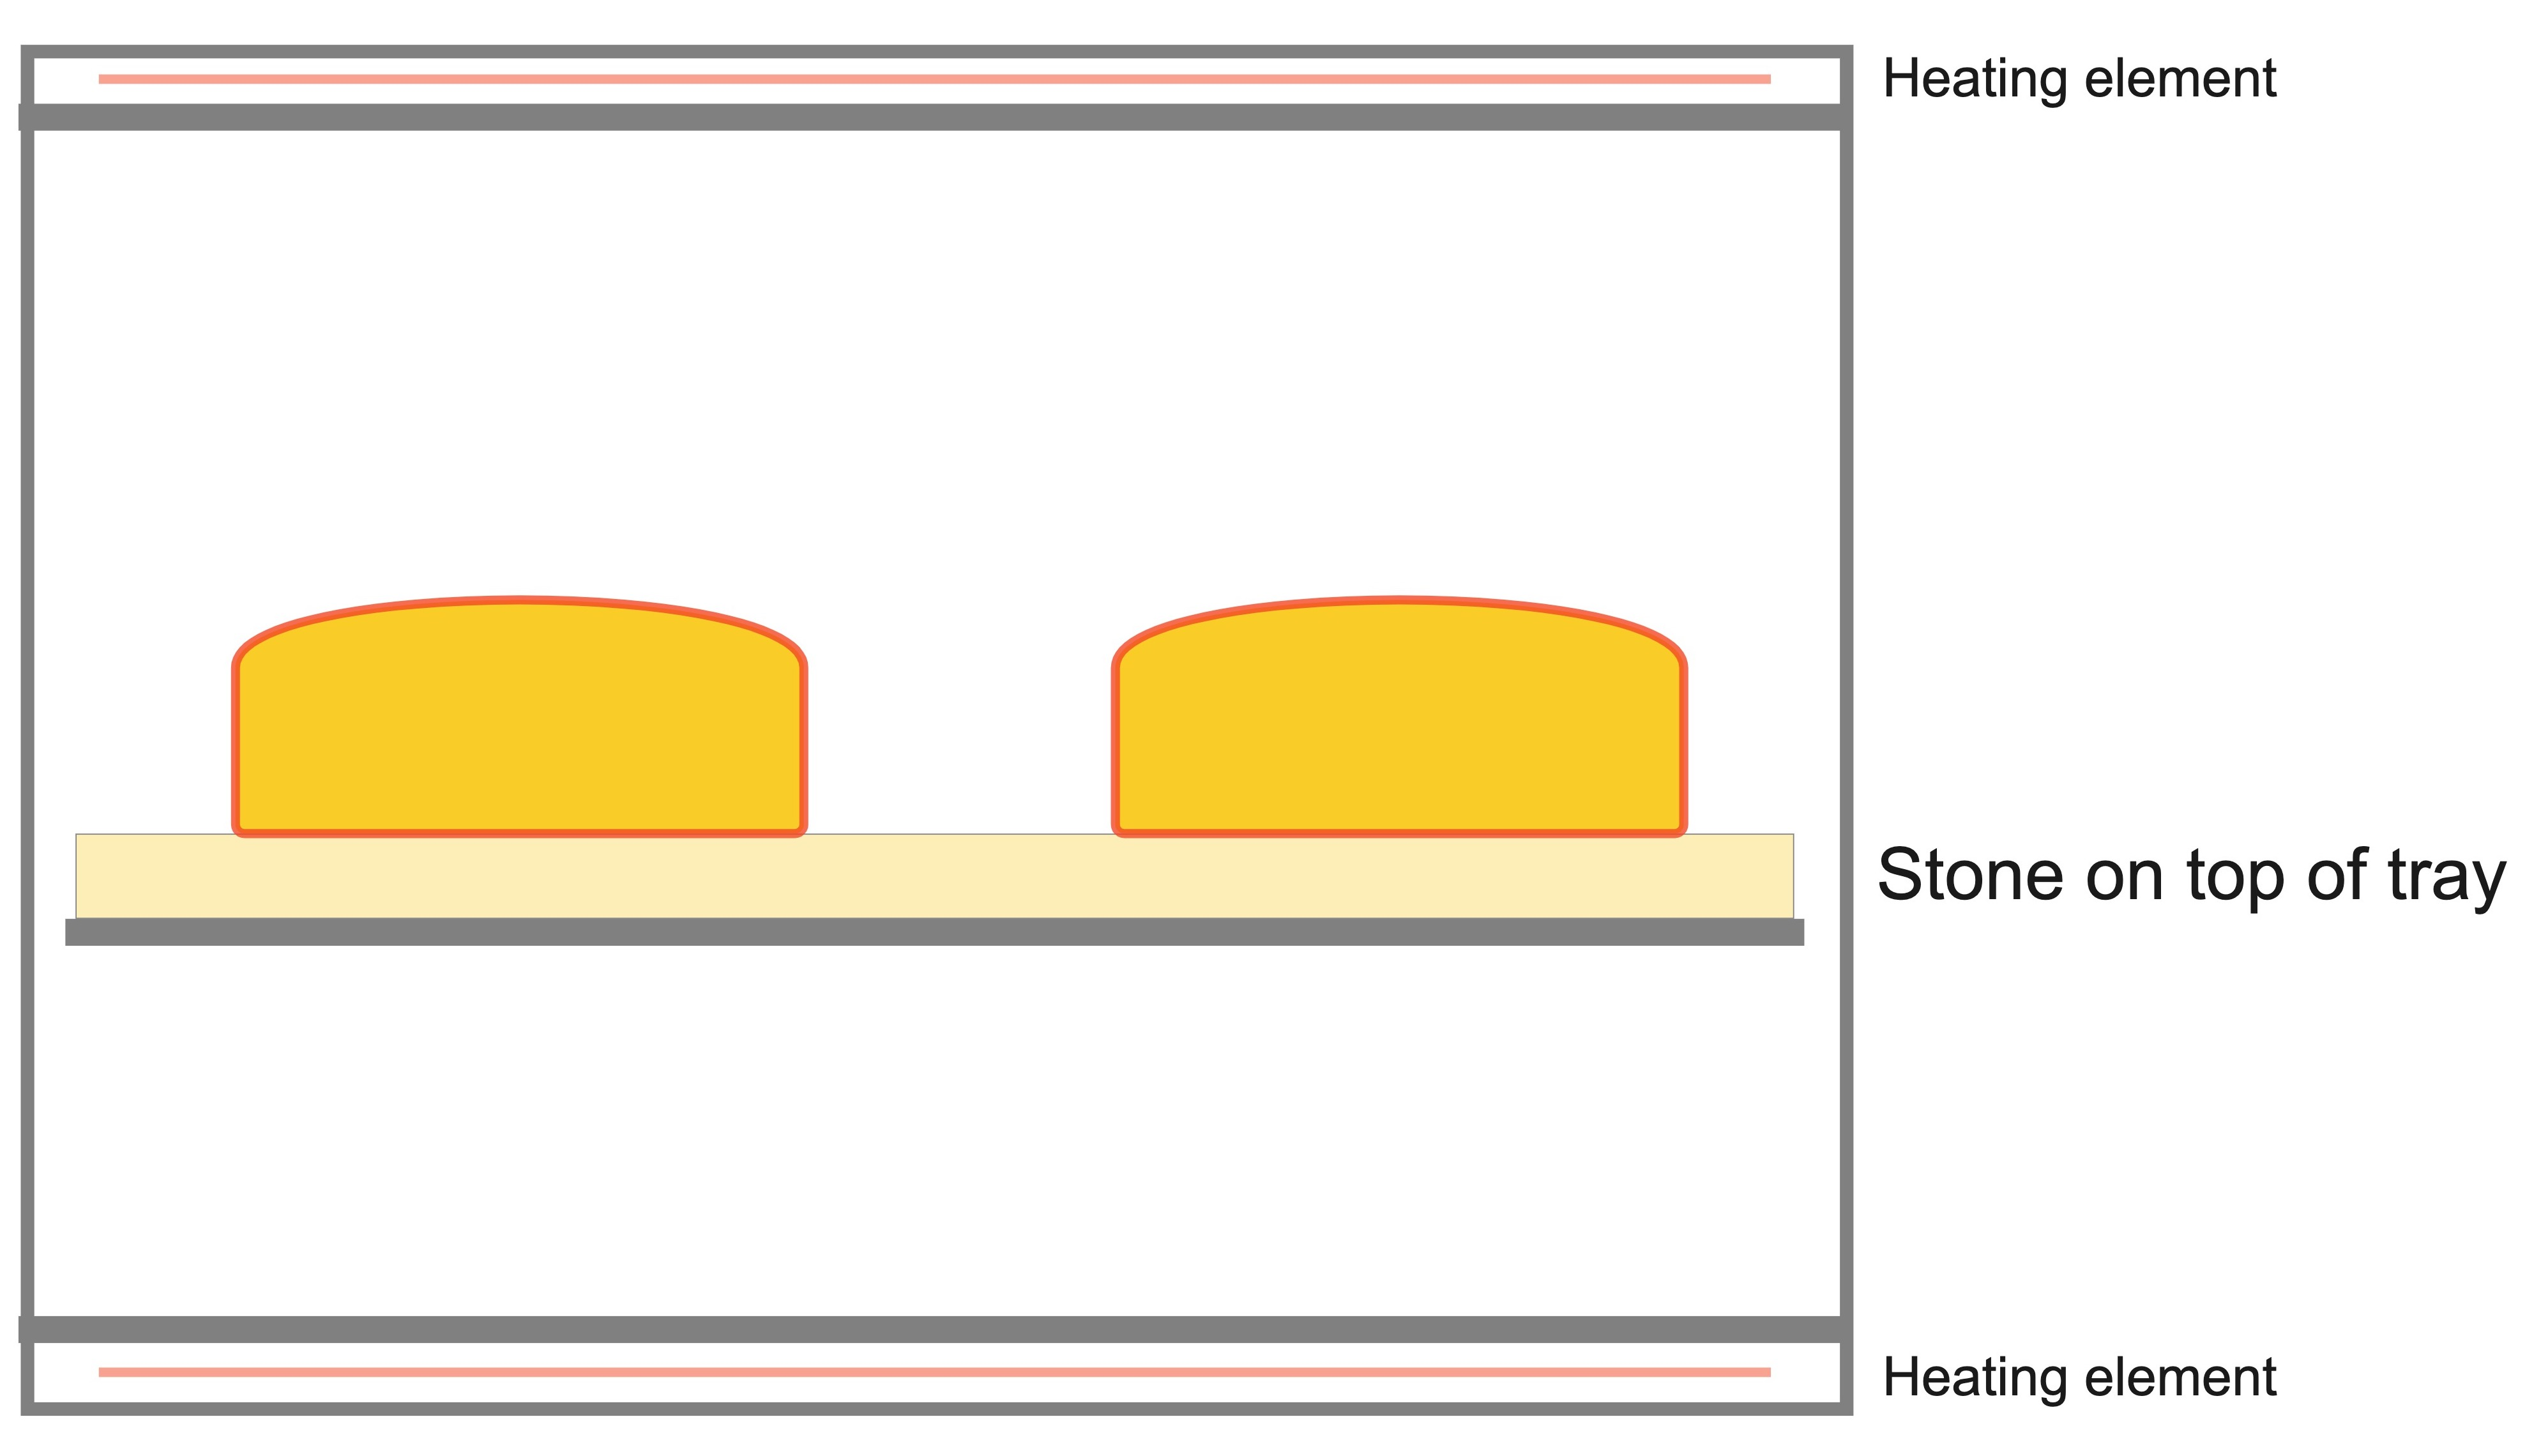
\includegraphics[width=\textwidth]{baking-process-stage-2.jpg}
  \caption{The second stage of the bake is done without steam to build
  a thicker darker crust}
\end{figure}

When not steaming enough you will notice that the scoring
incisions do not properly open up during the bake. They stay
closed as the dough is unable to push through the crust.

Furthermore a common sign is, that you have larger pockets
of air towards the crust of your dough. As the dough increases
vertically expansion is halted by the crust. The pockets
of air converge into larger pockets as pressure increases.
This can also happen when you are baking at a too hot temperature.

The more you steam the softer your dough's crust is. You will never
enter the maillard and caramelization stage. This
is the reason why the source of steam is removed
for the second stage of the bake. No more expansion can
happen and you can focus on building a crust. If you
would like a soft crust you can steam your dough all the
way.

\begin{figure}[!htb]
  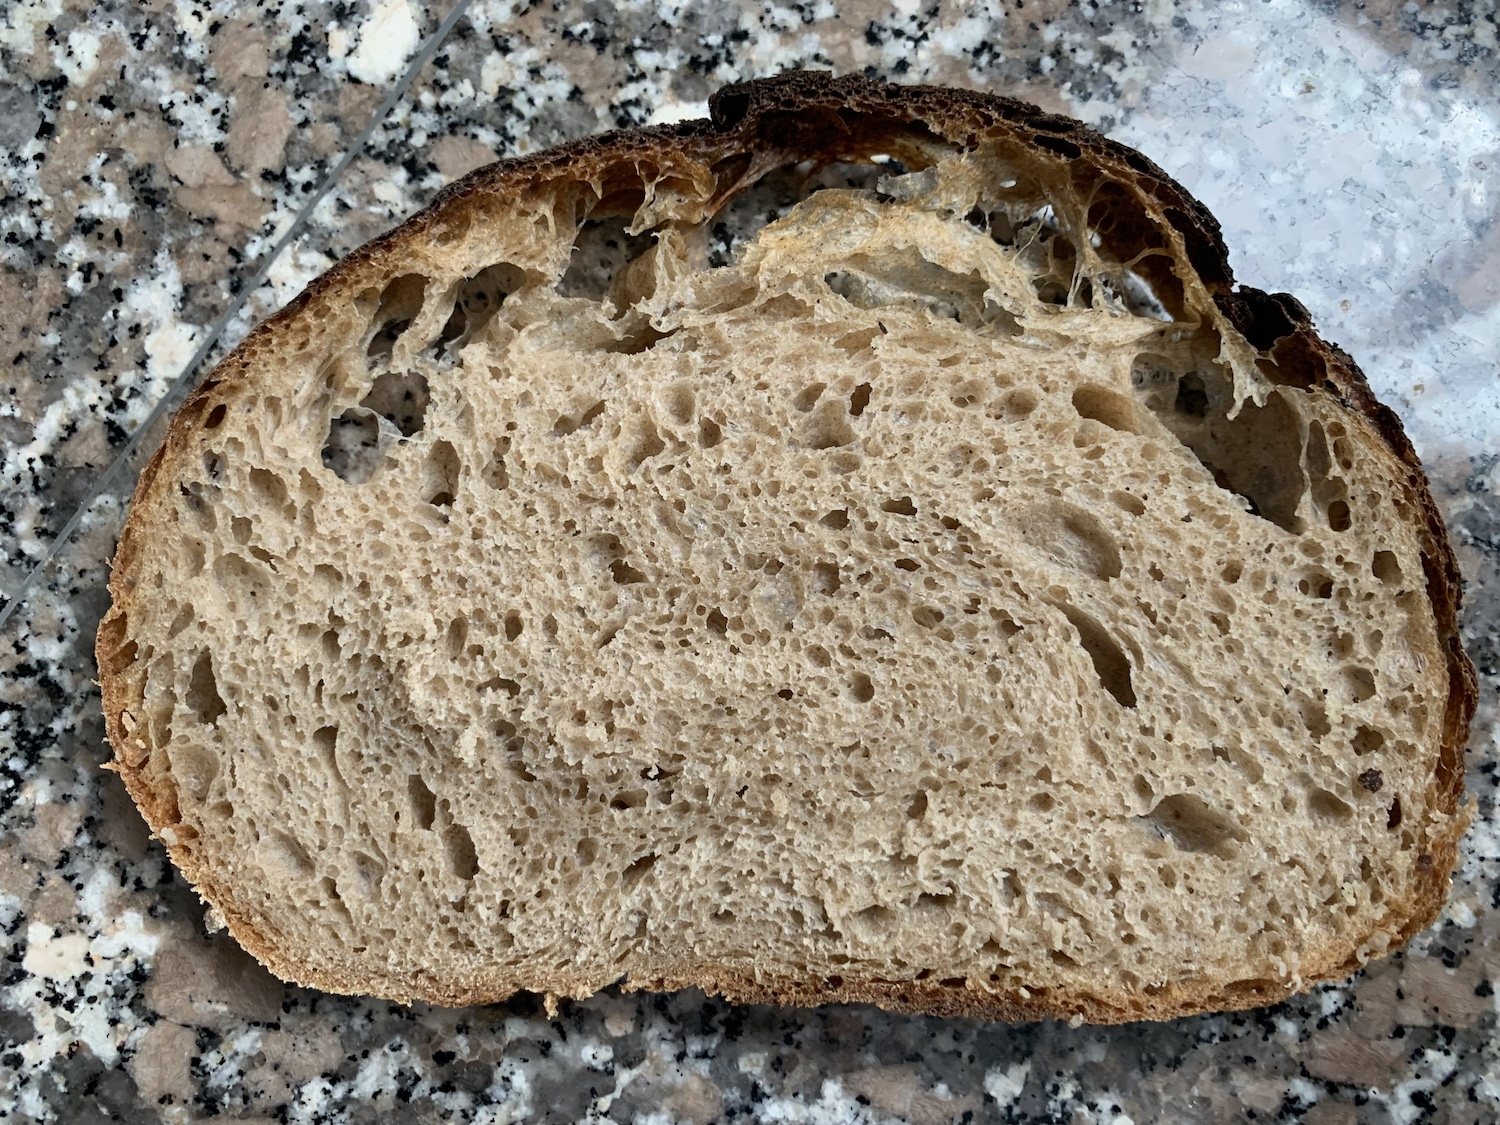
\includegraphics[width=\textwidth]{baking-too-hot.jpeg}
  \caption{A submission by Karomizu showing a bread that has been baked
  at a too hot temperature or with too little steam. Note the large
  pockets of air towards the crust. They are a typical indicator.}
\end{figure}

\section{Dutch ovens}

Dutch ovens are an ideal way to bake with a lot of
steam. They are not fully sealed. Regardless though
as water evaporates from your dough it will create a steamy
environment allowing your dough to rise. It really
makes baking in a home oven very easy.

When using a dutch oven make sure to preheat it properly,
this way your dough will not stick to it. You can also
use additional semolina flour or parchment paper. Another
good trick is to spritz your dough with a bit of water.
To create more steam you could also place a small ice cube
next to your main dough.

I have been using a dutch oven myself for a long time. They
have issues though. They are relatively heavy. It is dangerous
to operate hot cast iron ovens. Especially when working with steam
you have to be very careful.  Furthermore
they are expensive to buy. Then your dutch oven is made out
of cast iron you have to season it from time to time. This takes
time.

The biggest disadvantage though is
capacity. You can only bake a single bread at the
same time. In many cases it makes sense to bake multiple
loaves in one go. It makes the whole process more
efficient as you have to knead less per loaf. The time it
takes to make one bread significantly reduces. Furthermore
you don't require as much energy. You don't have
to preheat your oven twice for each individual loaf.


\section{Inverted tray method}

The inverted tray method simulates a dutch oven.
By placing another tray on top of your dough the steam
created from the dough and water source stays
around your dough.

\begin{figure}[!htb]
  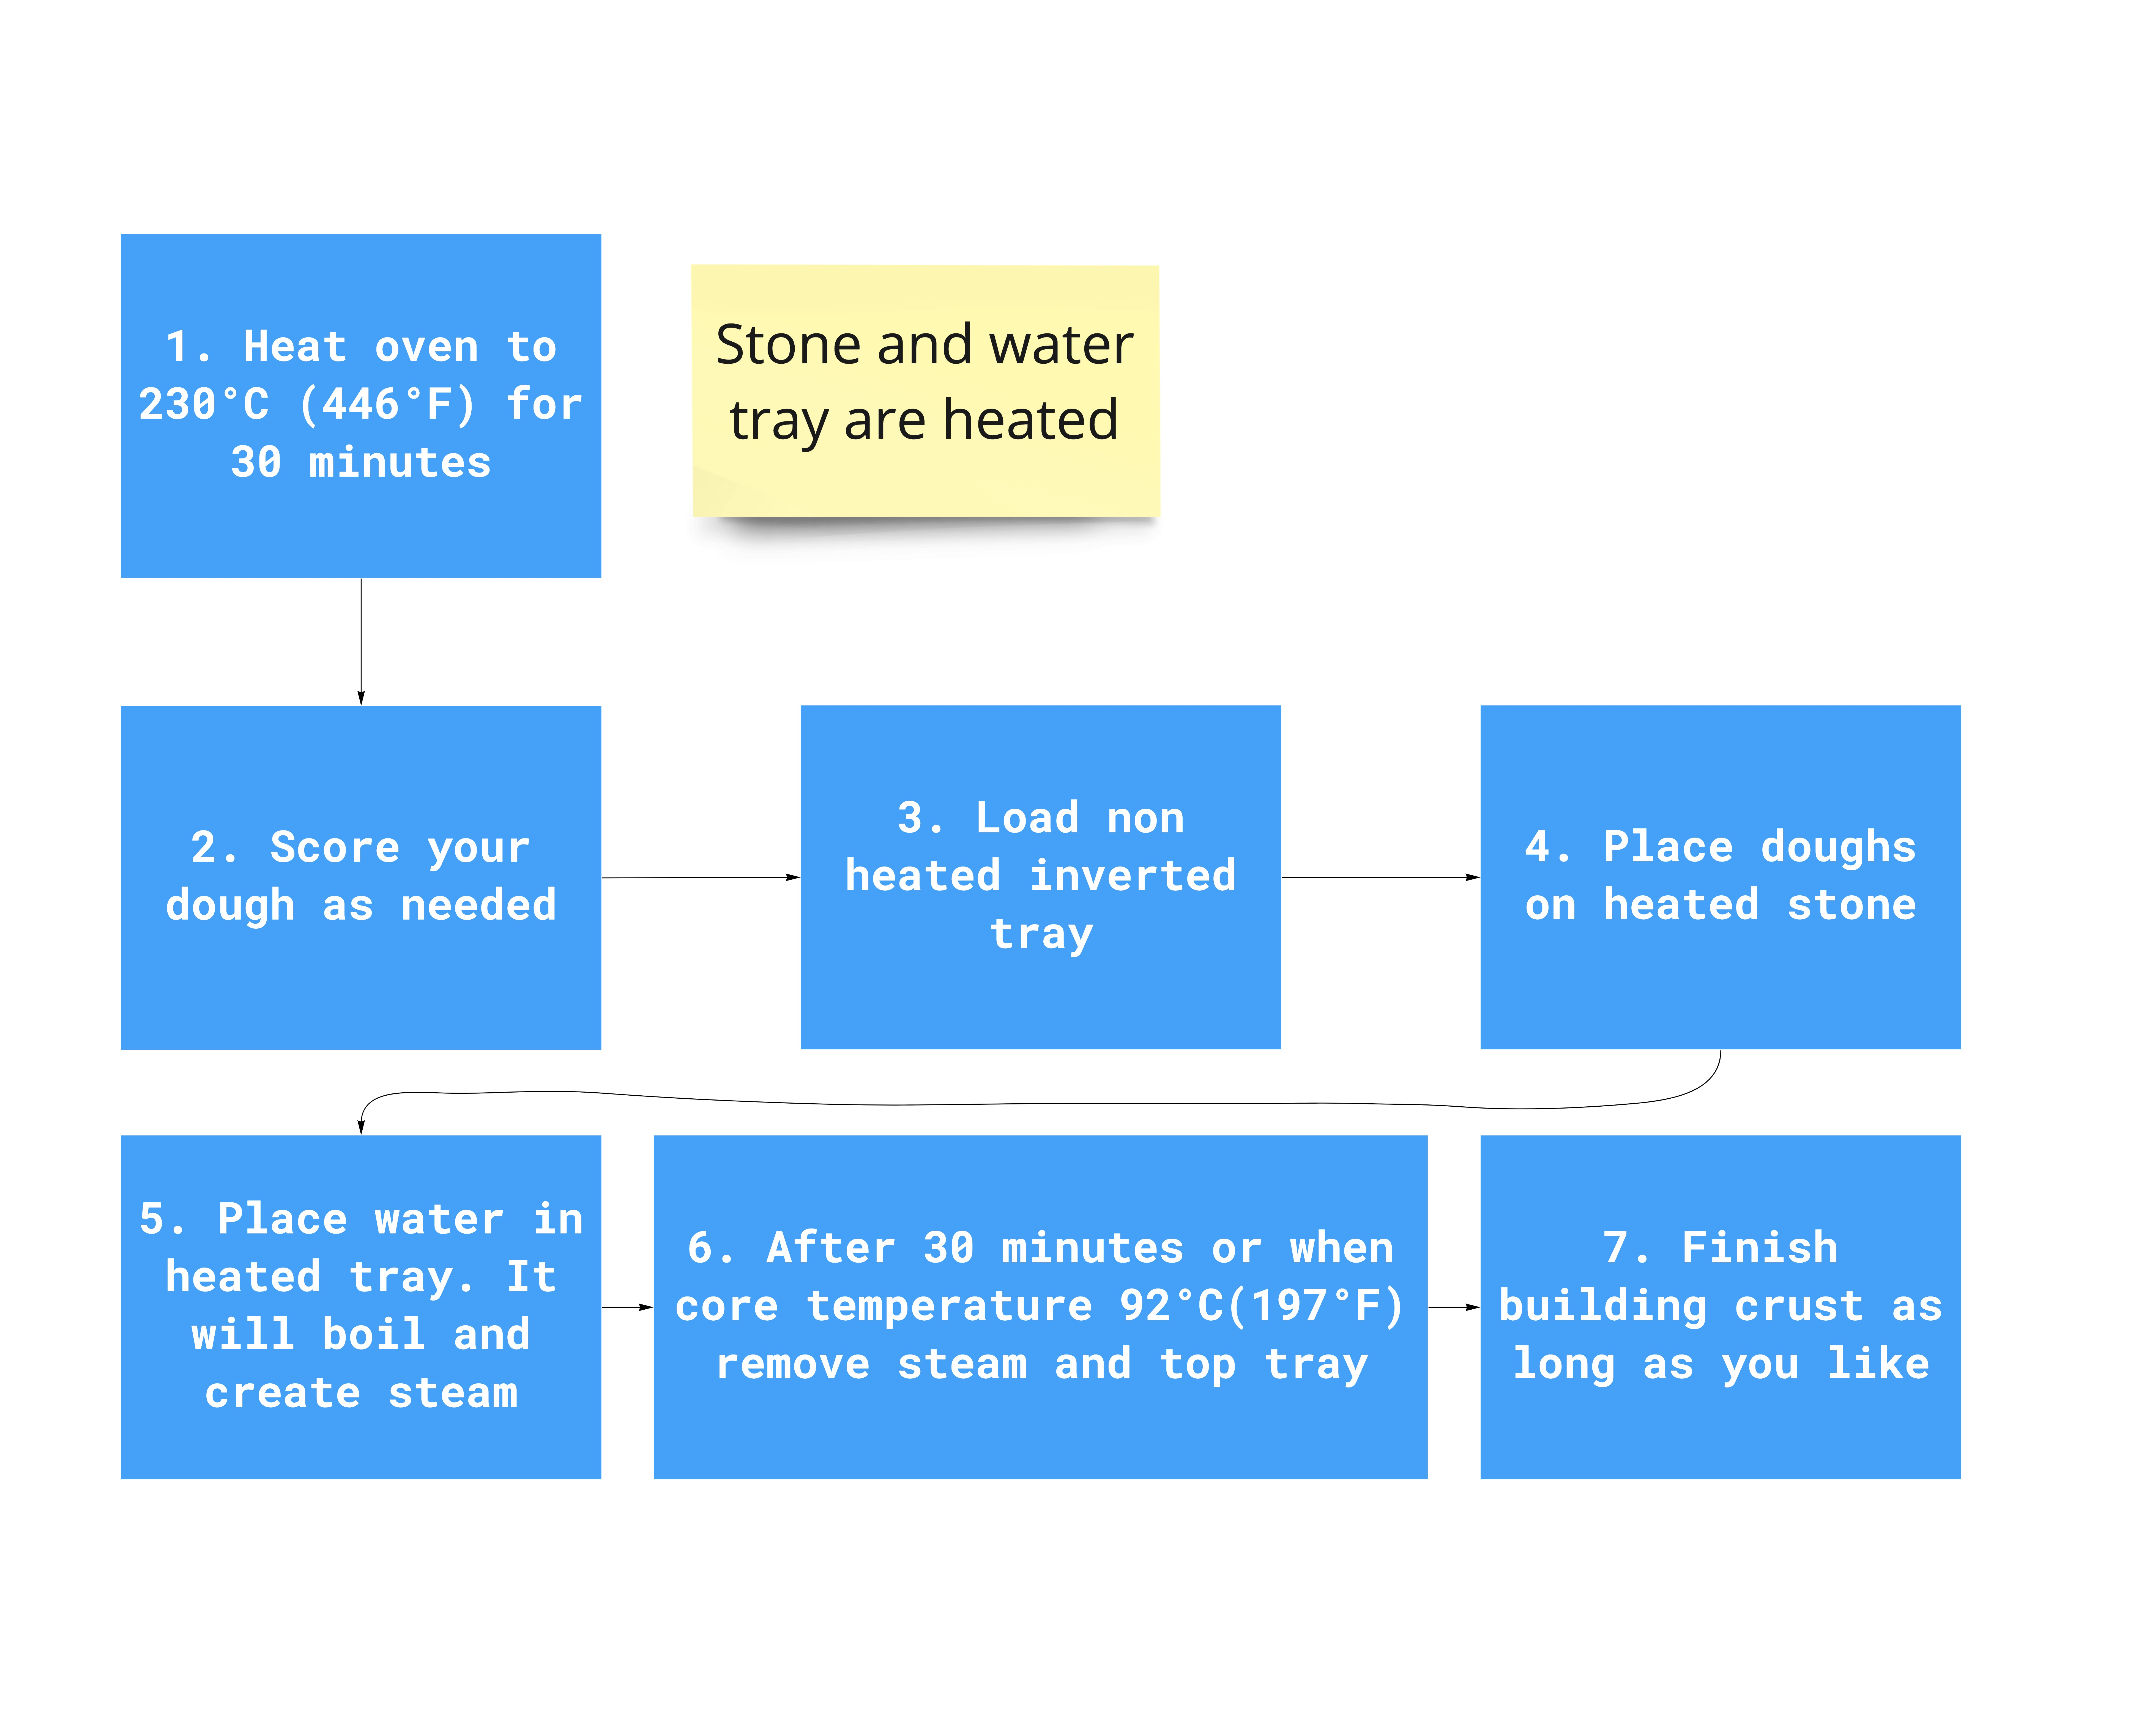
\includegraphics[width=\textwidth]{baking-process-overview.jpg}
  \caption{The full inverted tray method process}
\end{figure}


The biggest advantage of this method compared to the
dutch oven is scalability. You can bake multiple loaves
at the same time. In my case that is around 2 freestanding
loaves and 4 loaves in a loaf pan.

For the inverted tray you will need the following tools:
\begin{itemize}
\item 2 trays
\item 1 heat resistant bowl
\item Boiling water
\item Oven gloves
\item Optional parchment paper
\end{itemize}

\begin{figure}[!htb]
  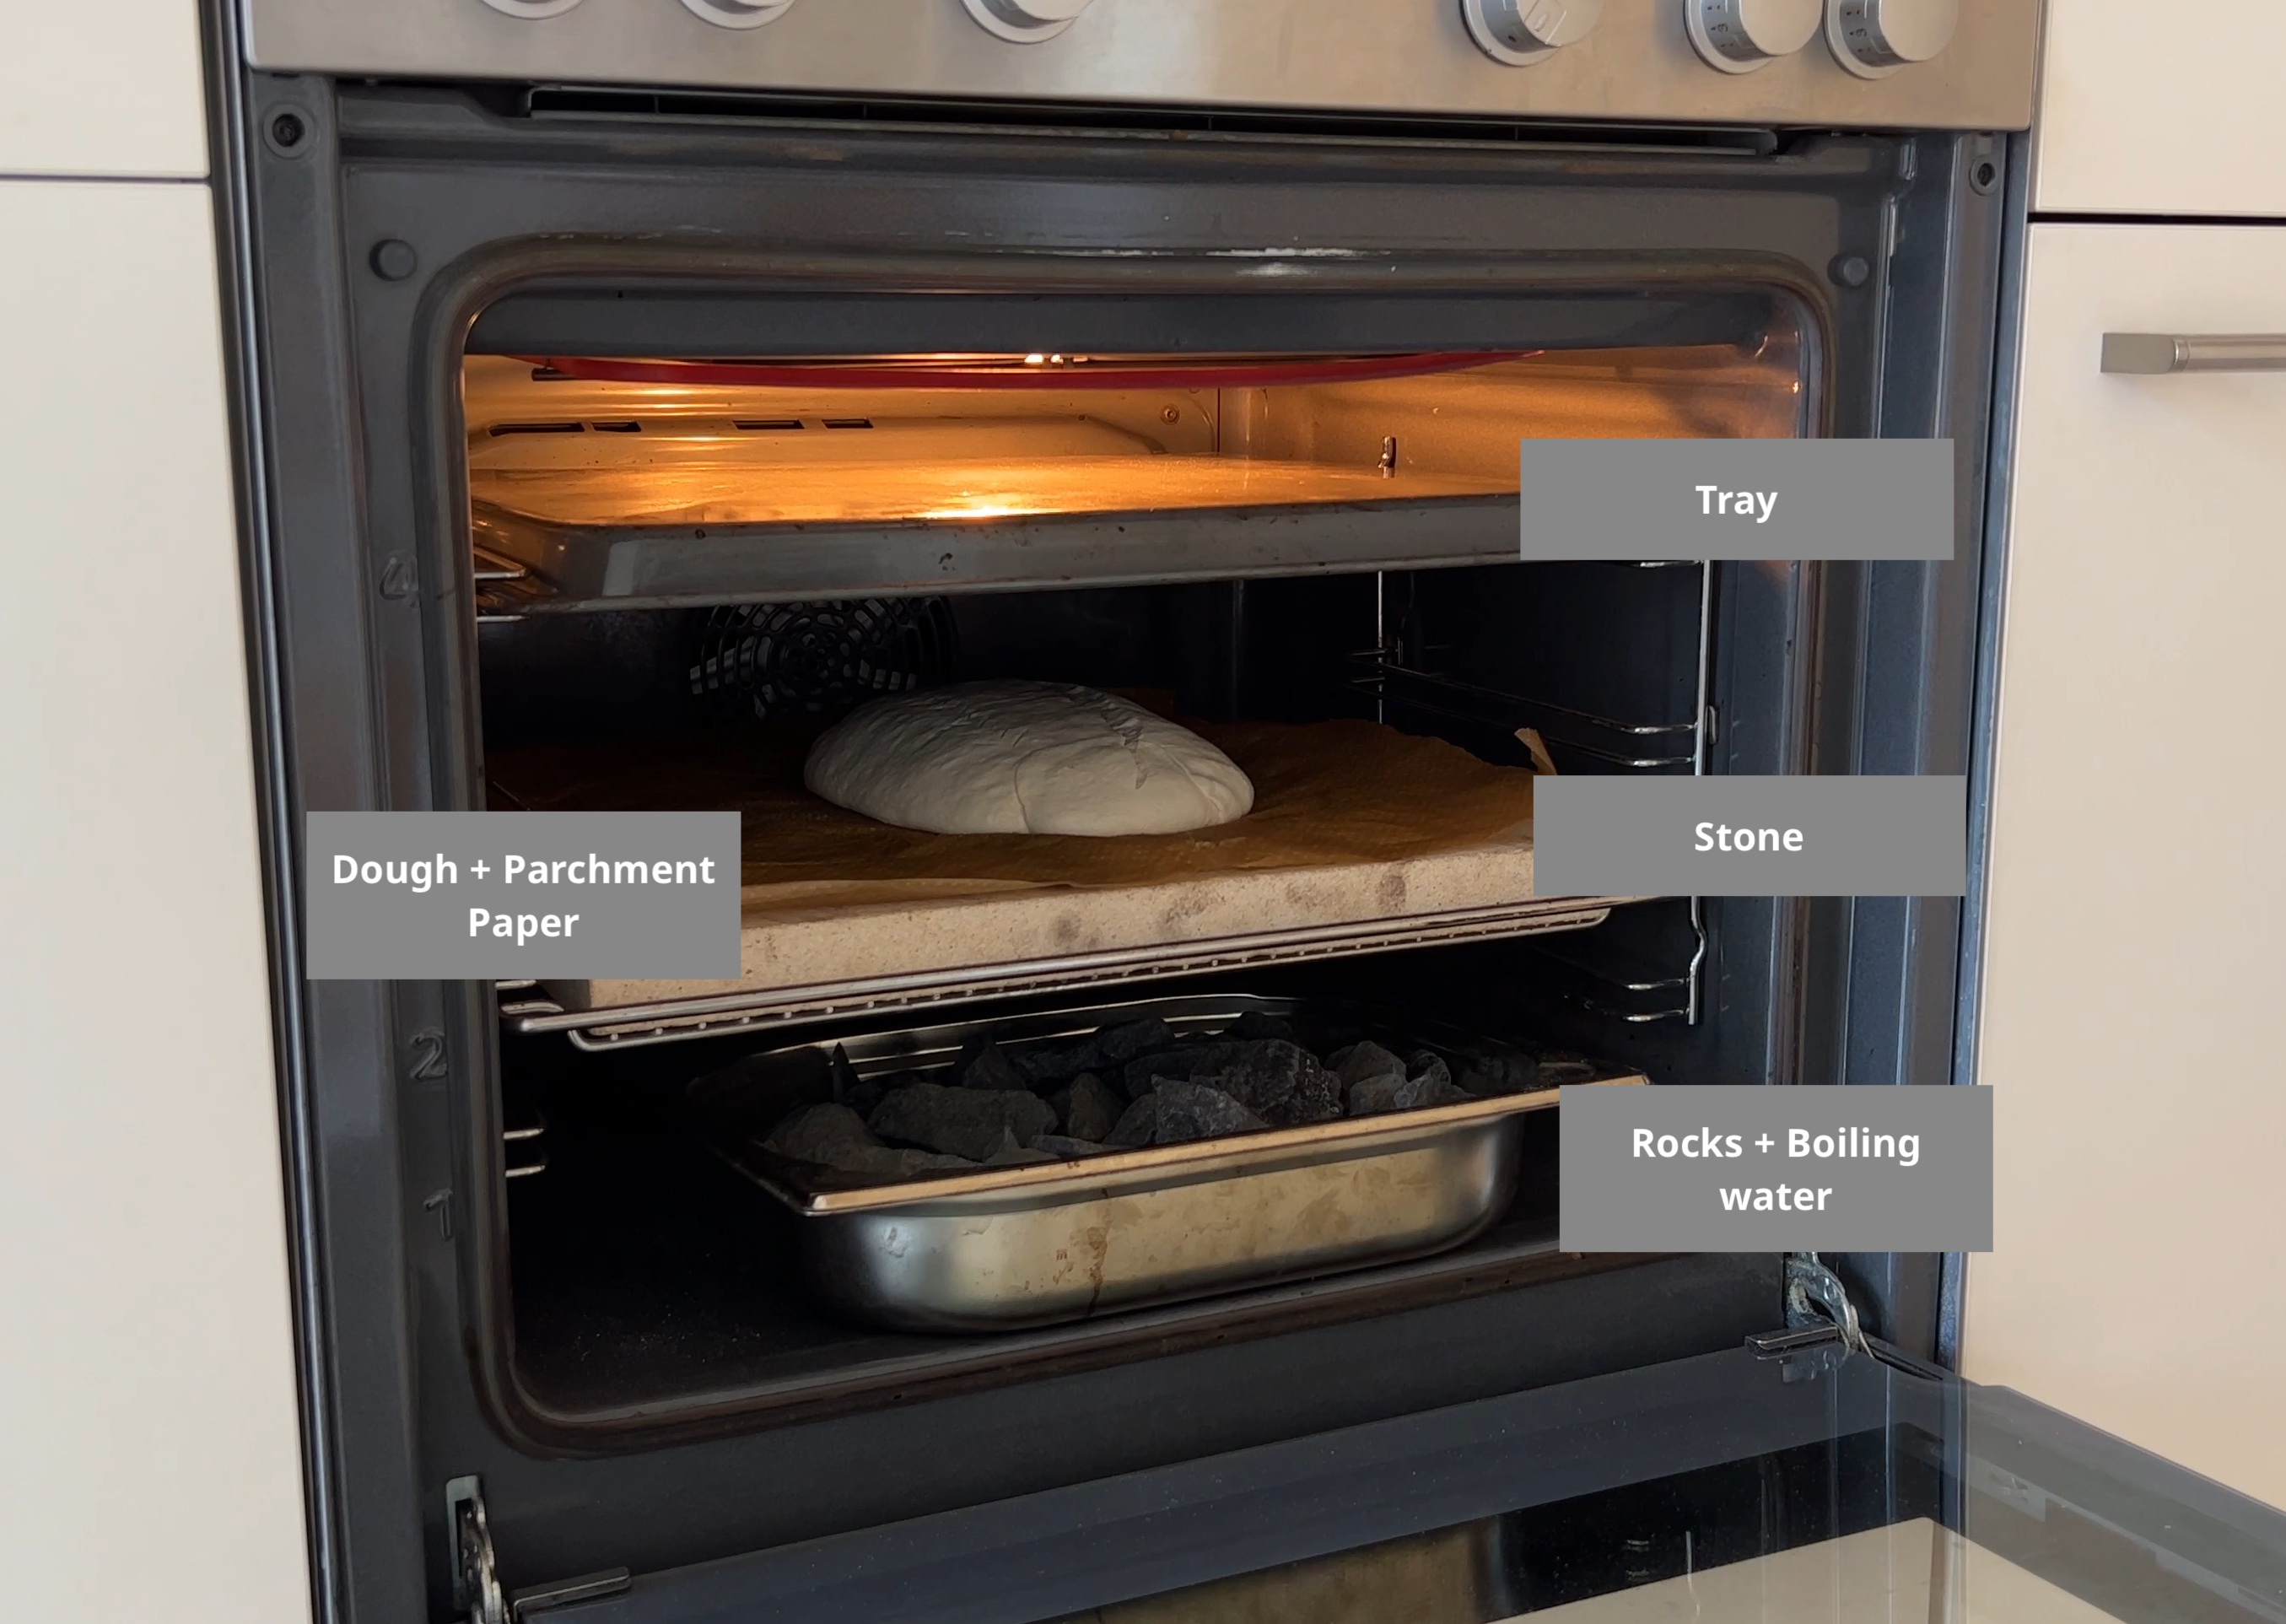
\includegraphics[width=\textwidth]{baking-example.jpg}
  \caption{My home oven setup}
\end{figure}

These are the steps to follow with the inverted tray method
\begin{enumerate}
\item Preheat the the oven to around 230°C (446°F)
Preheat one of the trays
\item Bring water to boil
\item Place your doughs on a piece of parchment paper. You
can also place each on a tiny piece of parchment paper
this makes loading the dough easier. If you don't
have it or don't want to use it, you can opt for 
semolina flour. It helps to make the tray non stick
\item Take out your hot tray and place it
on a cooling rack, or on something else that
is heat resistant
\item Score your doughs
\item Place your doughs on the hot tray
\item Place the cold tray in your oven in an inverted position
\item Move your hot tray including the loaves back
to the oven
\item Place the boiling water in the heat resistant
water bowl. I have added rocks to it, it helps
to improve the steam even further. This is optional
\item Close the oven
\item After 30 minutes remove the top tray. Also remove the bowl with water
\item Finish baking your bread until you have reached your desired
crust color. In my case this is another 15-25 minutes typically.
\end{enumerate}

\section{Conclusions}

\begin{table}[]
  \centering
  \resizebox{\textwidth}{!}{%
  \begin{tabular}{|l|l|l|l|}
  \hline
  \textbf{Oven type}                                                         & \textbf{Plain (no tools)} & \textbf{Inverted tray} & \textbf{Dutch oven} \\ \hline
  Gas                                                                        & No                        & No                     & Yes                 \\ \hline
  \begin{tabular}[c]{@{}l@{}}Convection\\ (Fan always on)\end{tabular}       & No                        & No                     & Yes                 \\ \hline
  \begin{tabular}[c]{@{}l@{}}Convection\\ (Fan can be disabled)\end{tabular} & No                        & Yes                    & Yes                 \\ \hline
  Steam                                                                      & Yes                       & Yes                    & Yes                 \\ \hline
  \end{tabular}%
  }
  \caption{An overview of ovens and their different baking methods}
\end{table}

Depending on your home oven a different method
of steaming should be used. Generally most ovens
are made to vent out most of the steam during the
bake. They are typically not fully closed. During
baking you want to dry out whatever you are baking.
This is ideal if you are baking vegetables and
want them to dry out. For baking though this is
highly problematic. As described earlier, you
want there to be as much steam as possible.

If you are using a gas based oven the only option
is to utilize a dutch oven. The same is true when you
are using a convection oven with a fan that
can not be disabled. When using a convection
oven with a fan that can be turned off, you can
opt to use the cost efficient inverted tray
method.

If you are in the luxurious
position to own a steam oven, things are easier.
Just activate the steam function and you are
good to go. Placing an additional tray on top of your
dough during the bake helps to bake with indirect
heat. You remain in the gel zone longer and
will experience more oven spring.